%begin detailed
\section{Основные понятия}
\begin{frame}{Labelled Transition Systems}

Понятие бисимуляции возникло в контексте систем размеченных переходов (LTS).

\begin{block}{\bf Определение}
Labelled Transition System --- тройка $\langle S, \Sigma, Q\rangle$, где $S$ --- множество состояний, $\Sigma$ --- множество меток, $Q$ --- множество переходов (троек из $S\times\Sigma\times S$). 
\end{block} % descriptive documentation

LTS похожи на конечные автоматы, но допускают бесконечные множества $S$ и $Q$. Кроме того, в LTS нет начальных и финальных состояний. % overall documentation 

\begin{exampleblock}{}
Трансформационный моноид также строится в контексте LTS, то есть без учёта финальности состояний. Поэтому из ДКА, по которому строится трансформационный моноид, предварительно удаляются все ловушки, иначе в нём могут появиться правила переписывания, не имеющие никакого отношения к языку ДКА.
\end{exampleblock}% advanced documentation % overall documentation
\end{frame}

\begin{frame}{Симуляция и бисимуляция}
\vspace*{-5pt}
\begin{block}{\bf Определение}
Если $\precsim$ --- симуляция для LTS = $\langle S, \Sigma, Q\rangle$, то
\[\forall p,q\in S(p\precsim q \logimpl (\exists p',a((p\transit{a} p')\logimpl\exists q'(q\transit{a}q'\logand p'\precsim q'))\]
\end{block} % descriptive documentation

Неформально можно считать, что если $p\precsim q$, то множество путей в LTS, стартующих в $p$, вкладывается в множество путей, начинающихся в $q$.  % descriptive documentation

\vspace*{-5pt}
\begin{block}{\bf Определение}
Если одновременно выполняются условия $p\precsim q$ и $q\precsim p$, то говорят, что $p$ и $q$ находятся в отношении бисимуляции (обозначается $p\sim q$).   
\end{block}  % descriptive documentation
{Бисимуляция состояний в единственной LTS легко обобщается и на бисимуляцию между двумя разными LTS. Поскольку в них нет начальных состояний, и они не обязаны быть связными, можно рассматривать несколько LTS как одну LTS с несколькими компонентами и искать бисимуляцию между элементами этих компонент.}  % overall documentation
\end{frame}

\section{Бисимилярность НКА}
\begin{frame}{Бисимилярность НКА}
Чтобы определить отношение бисимуляции на конечных автоматах, к отношению бисимуляции на LTS нужно добавить ограничения на бисимуляцию начальных и конечных состояний. Более точно, для бисимуляции НКА $\Aut_1$ и $\Aut_2$ необходимы следующие условия: % descriptive documentation
\begin{enumerate}
\item каждому состоянию $\Aut_1$ бисимилярно состояние $\Aut_2$, и наоборот;
\item стартовому состоянию $\Aut_1$ бисимилярно стартовое состояние $\Aut_2$;
\item каждому финальному состоянию $\Aut_1$ бисимилярно финальное состояние $\Aut_2$, и наоборот.
\end{enumerate} % descriptive documentation

\begin{exampleblock}{\bf Лемма}
Бисимилярные НКА распознают равные языки. Это следует из бисимилярности их стартовых состояний (назовём их $q_0$ и $q'_0$) и того факта, что любой путь из $q_0$ в финальное состояние в таком НКА соответствует какому-нибудь пути из $q'_0$ в бисимилярном ему.
\end{exampleblock} % overall documentation

\end{frame}

\begin{frame}{Пример бисимилярных НКА} % Bisimilar
\vspace*{-5pt}
{Рассмотрим следующие два автомата, распознающие язык $a\star b$.} % specific documentation

\smallskip
\begin{minipage}{0.45\textwidth}
\begin{tabular}{c}
Автомат $\Aut_1$:\\\\ 
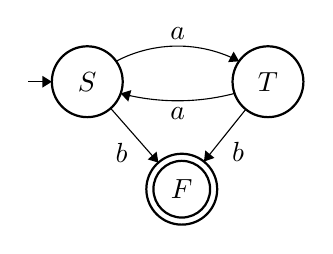
\begin{tikzpicture}[scale=0.15] % first automaton placeholder
\tikzstyle{every node}+=[inner sep=0pt]
\draw [black,thick] (19.2,-19.7) circle (3);
\draw (19.2,-19.7) node {$S$};
\draw [black,thick] (34.5,-19.7) circle (3);
\draw (34.5,-19.7) node {$T$};
\draw [black,thick] (27.2,-28.8) circle (3);
\draw (27.2,-28.8) node {$F$};
\draw [black,thick] (27.2,-28.8) circle (2.4);
\draw [black] (21.18,-21.95) -- (25.22,-26.55);
\fill [black] (25.22,-26.55) -- (25.07,-25.62) -- (24.32,-26.28);
\draw (22.66,-25.7) node [left] {$b$};
\draw [black] (32.62,-22.04) -- (29.08,-26.46);
\fill [black] (29.08,-26.46) -- (29.97,-26.15) -- (29.19,-25.52);
\draw (31.41,-25.67) node [right] {$b$};
\draw [black] (21.638,-17.967) arc (117.72671:62.27329:11.202);
\fill [black] (32.06,-17.97) -- (31.59,-17.15) -- (31.12,-18.04);
\draw (26.85,-16.18) node [above] {$a$};
\draw [black] (31.672,-20.69) arc (-75.24187:-104.75813:18.927);
\fill [black] (22.03,-20.69) -- (22.67,-21.38) -- (22.93,-20.41);
\draw (26.85,-21.81) node [below] {$a$};
\draw [black] (14.2,-19.7) -- (16.2,-19.7);
\fill [black] (16.2,-19.7) -- (15.4,-19.2) -- (15.4,-20.2);
\end{tikzpicture}
\end{tabular}
\end{minipage} 
\quad
\begin{minipage}{0.45\textwidth}
\begin{tabular}{c}
Автомат $\Aut_2$:\\\\ 
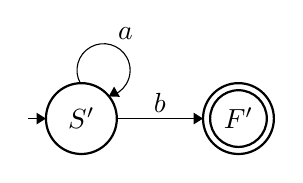
\begin{tikzpicture}[scale=0.15] % second automaton placeholder
\tikzstyle{every node}+=[inner sep=0pt]
\draw [black,thick] (51.6,-19.1) circle (3);
\draw (51.6,-19.1) node {$S'$};
\draw [black,thick] (64.9,-19.1) circle (3);
\draw (64.9,-19.1) node {$F'$};
\draw [black,thick] (64.9,-19.1) circle (2.4);
\draw [black] (51.516,-16.113) arc (209.34315:-78.65685:2.25);
\draw (55.34,-12.46) node [above] {$a$};
\fill [black] (53.92,-17.22) -- (54.86,-17.26) -- (54.37,-16.39);
\draw [black] (47.1,-19.1) -- (48.6,-19.1);
\fill [black] (48.6,-19.1) -- (47.8,-18.6) -- (47.8,-19.6);
\draw [black] (54.6,-19.1) -- (61.9,-19.1);
\fill [black] (61.9,-19.1) -- (61.1,-18.6) -- (61.1,-19.6);
\draw (58.25,-18.6) node [above] {$b$};
\end{tikzpicture}
\end{tabular}
\end{minipage} 

\smallskip
\begin{minipage}{0.45\textwidth}
Между ними есть бисимуляция:
\[\bigl\{\langle S, S'\rangle, \langle T, S'\rangle, \langle F, F'\rangle\bigr\}\] % bisimilarity pairs placeholder
{Состояния $S$ и $T$ бисимилярны одному и тому же состоянию $S'$ --- это означает, что множества путей из них в $\Aut_1$ неразличимы.} % specific documentation
\end{minipage}
\;
\begin{minipage}{0.45\textwidth}
\begin{center}
\begin{tikzpicture}[scale=0.12] % bisimilarity demo placeholder
\tikzstyle{every node}+=[inner sep=0pt]
\draw [green80,very thick,fill=green!20] (19.6,-19.1) circle (3);
\draw (19.6,-19.1) node {$S$};
\draw [green80,very thick,fill=green!20] (34.1,-19.1) circle (3);
\draw (34.1,-19.1) node {$T$};
\draw [blue,very thick,fill=teal!20] (27.2,-28.8) circle (3);
\draw (27.2,-28.8) node {$F$};
\draw [blue,thick] (27.2,-28.8) circle (2.4);
\draw [green80,very thick,fill=green!20] (51.6,-19.1) circle (3);
\draw (51.6,-19.1) node {$S'$};
\draw [blue,very thick,fill=teal!20] (51.6,-28.8) circle (3);
\draw (51.6,-28.8) node {$F'$};
\draw [blue,thick] (51.6,-28.8) circle (2.4);
\draw [blue, thick] (21.45,-21.46) -- (25.35,-26.44);
\fill [blue] (25.35,-26.44) -- (25.25,-25.5) -- (24.46,-26.12);
\draw (22.83,-25.37) node [left] {$b$};
\draw [blue, thick] (32.36,-21.54) -- (28.94,-26.36);
\fill [blue] (28.94,-26.36) -- (29.81,-25.99) -- (29,-25.41);
\draw (31.24,-25.32) node [right] {$b$};
\draw [green80,thick] (21.994,-17.31) arc (118.38381:61.61619:10.216);
\fill [green80] (31.71,-17.31) -- (31.24,-16.49) -- (30.76,-17.37);
\draw (26.85,-15.58) node [above] {$a$};
\draw [green80,thick] (31.286,-20.129) arc (-74.949:-105.051:17.083);
\fill [green80] (22.41,-20.13) -- (23.06,-20.82) -- (23.32,-19.85);
\draw (26.85,-21.21) node [below] {$a$};
\draw [black] (14.6,-19.1) -- (16.6,-19.1);
\fill [black] (16.6,-19.1) -- (15.8,-18.6) -- (15.8,-19.6);
\draw [blue, thick] (51.6,-22.1) -- (51.6,-25.8);
\fill [blue] (51.6,-25.8) -- (52.1,-25) -- (51.1,-25);
\draw (52.1,-23.95) node [right] {$b$};
\draw [green80,thick] (51.516,-16.113) arc (209.34315:-78.65685:2.25);
\draw (55.34,-12.46) node [above] {$a$};
\fill [green80] (53.92,-17.22) -- (54.86,-17.26) -- (54.37,-16.39);
\draw [red, ultra thick, dashed] (21.188,-16.559) arc (143.21235:36.78765:17.995);
\draw [red, ultra thick, dashed] (36.961,-18.205) arc (103.87647:76.12353:24.554);
\draw [red, ultra thick, dashed] (30.098,-28.028) arc (102.8591:77.1409:41.795);
\draw [black] (47.1,-19.1) -- (48.6,-19.1);
\fill [black] (48.6,-19.1) -- (47.8,-18.6) -- (47.8,-19.6);
\end{tikzpicture}
\end{center}
\end{minipage} 
\end{frame}

% counterexample documentation - frame
\begin{frame}{Бисимуляция и равенство}
В равных НКА состояния бисимилярны, однако только условия существования бисимуляции и биекции бисимилярных состояний недостаточно, чтобы гарантировать равенство. % возможно, стоит перенести в слайды про равенство НКА

\begin{exampleblock}{\bf Пример неравных бисимилярных НКА}
\textit{(автор примера: А.\,Д.\,Дельман)}

Следующие два автомата бисимилярны и имеют одинаковое число состояний, однако не равны:

\begin{center}
\begin{tikzpicture}[scale=0.15]
\tikzstyle{every node}+=[inner sep=0pt]
\draw [blue,very thick,fill=teal!20] (10.4,-18.9) circle (3);
\draw (10.4,-18.9) node {$q_0$};
\draw [green80,very thick,fill=green!20] (19.3,-13) circle (3);
\draw (19.3,-13) node {$q_1$};
\draw [violet80,very thick, fill=violet80!15] (19.3,-24.7) circle (3);
\draw (19.3,-24.7) node {$q_2$};
\draw [yellow80,very thick, fill=yellow!25] (31.2,-13) circle (3);
\draw (31.2,-13) node {$q_3$};
\draw [yellow80,thick] (31.2,-13) circle (2.4);
\draw [yellow80,very thick, fill=yellow!25] (31.2,-24.7) circle (3);
\draw (31.2,-24.7) node {$q_4$};
\draw [yellow80,thick] (31.2,-24.7) circle (2.4);
\draw [blue,very thick,fill=teal!20] (46.6,-18.9) circle (3);
\draw (46.6,-18.9) node {$q'_0$};
\draw [green80,very thick,fill=green!20] (55.9,-13) circle (3);
\draw (55.9,-13) node {$q'_1$};
\draw [violet80,very thick, fill=violet80!15] (55.9,-24.7) circle (3);
\draw (55.9,-24.7) node {$q'_2$};
\draw [yellow80,very thick, fill=yellow!25] (67.6,-13) circle (3);
\draw (67.6,-13) node {$q'_3$};
\draw [yellow80,thick] (67.6,-13) circle (2.4);
\draw [yellow80,very thick, fill=yellow!25] (67.6,-24.7) circle (3);
\draw (67.6,-24.7) node {$q'_4$};
\draw [yellow80,thick] (67.6,-24.7) circle (2.4);
\draw [black] (5.8,-18.9) -- (7.4,-18.9);
\fill [black] (7.4,-18.9) -- (6.6,-18.4) -- (6.6,-19.4);
\draw [black] (41.9,-18.9) -- (43.6,-18.9);
\fill [black] (43.6,-18.9) -- (42.8,-18.4) -- (42.8,-19.4);
\draw [black] (12.9,-17.24) -- (16.8,-14.66);
\fill [black] (16.8,-14.66) -- (15.86,-14.68) -- (16.41,-15.52);
\draw (13.85,-15.45) node [above] {$b$};
\draw [black] (12.91,-20.54) -- (16.79,-23.06);
\fill [black] (16.79,-23.06) -- (16.39,-22.21) -- (15.84,-23.04);
\draw (13.85,-22.3) node [below] {$b$};
\draw [black] (22.3,-13) -- (28.2,-13);
\fill [black] (28.2,-13) -- (27.4,-12.5) -- (27.4,-13.5);
\draw (25.25,-12.5) node [above] {$a$};
\draw [black] (21.44,-15.1) -- (29.06,-22.6);
\fill [black] (29.06,-22.6) -- (28.84,-21.68) -- (28.14,-22.39);
\draw (26.22,-18.37) node [above] {$c$};
\draw [black] (22.3,-24.7) -- (28.2,-24.7);
\fill [black] (28.2,-24.7) -- (27.4,-24.2) -- (27.4,-25.2);
\draw (25.25,-25.2) node [below] {$a$};
\draw [black] (49.13,-17.29) -- (53.37,-14.61);
\fill [black] (53.37,-14.61) -- (52.42,-14.61) -- (52.96,-15.46);
\draw (50.25,-15.45) node [above] {$b$};
\draw [black] (49.15,-20.49) -- (53.35,-23.11);
\fill [black] (53.35,-23.11) -- (52.94,-22.26) -- (52.41,-23.11);
\draw (50.25,-22.3) node [below] {$b$};
\draw [black] (58.191,-11.094) arc (118.31536:61.68464:7.504);
\fill [black] (65.31,-11.09) -- (64.84,-10.27) -- (64.37,-11.15);
\draw (61.75,-9.7) node [above] {$a$};
\draw [black] (64.974,-14.426) arc (-70.43174:-109.56826:9.626);
\fill [black] (64.97,-14.43) -- (64.05,-14.22) -- (64.39,-15.16);
\draw (61.75,-15.48) node [below] {$c$};
\draw [black] (58.9,-24.7) -- (64.6,-24.7);
\fill [black] (64.6,-24.7) -- (63.8,-24.2) -- (63.8,-25.2);
\draw (61.75,-25.2) node [below] {$a$};
\end{tikzpicture}
\end{center}
\end{exampleblock}

\end{frame}

%end detailed
\section{Слияние по бисимуляции}
%begin detailed
\begin{frame}{Бисимилярность состояний в НКА}

\begin{block}{\bf Определение}
Состояния $q_i$ $q_j$ в НКА $\Aut$ бисимилярны ($q_i\sim_{\Aut} q_j$), если они связаны LTS-бисимуляцией и имеют одинаковую финальность в $\Aut$.
\end{block} % descriptive documentation

\begin{itemize}
\item С учётом определения выше, бисимуляцию НКА можно переформулировать как отношение бисимуляции состояний НКА такое, что стартовые состояния бисимилярны. 
\item Отношение $\sim_{\Aut}$ имеет важное свойство: бисимилярные состояния в автомате можно объединить без изменения его семантики. Это преобразование часто позволяет существенно упростить НКА.
\end{itemize} % overall documentation

\begin{exampleblock}{\bf Пример}
Все состояния-ловушки в любом полном автомате (т.е. с явно присутствующими переходами по всем буквам алфавита) бисимилярны друг другу. Все финальные состояния без переходов из них (кроме как в ловушки) также бисимилярны. 
\end{exampleblock} % overall documentation

\end{frame}

%end detailed
\begin{frame}{Преобразование $\MergeBisim\TypeIs\NFATYPE\to\NFATYPE$} % MergeBisim
	Исходный автомат:

	%template_oldautomaton

	Итоговый автомат:

	%template_result

	Классы эквивалентности по бисимуляции:

	%template_equivclasses

%\smallskip
%{Бисимуляция: $\Bigl\{\bigl\{q_3,q_6\bigr\},\displaystyle\bigcup_{i\neq 3\logand i\neq 6}\bigl\{q_i\bigr\}\Bigr\}$} % bisimulation set placeholder

%{Кроме $q_3$ и $q_6$, все состояния не бисимилярны никаким другим. Например, $q_1\not\sim q_5$, поскольку $q_1\transit{b}q_0$, $q_5\transit{b}q_6$, но $q_0\transit{a} q_1$ (и $q_1$ --- не финальное), а из $q_6$ есть переход только в финальное состояние $q_2$.}
% specific documentation
\end{frame}
